\customHeader{1}{Splitting the Dataset}
\label{06_splitting_the_dataset}

As mentioned at the end of \headerName{} \ref{vsi_results_of_preprocessing}, after preprocessing, we obtain eight datasets for binary \textclassification{}. For each dataset, we produce seven splits, two for training using \finetuning{} and five for training using \gls{pet}.


The simplest splitting strategy is the one for \finetuning{} on an unbalanced dataset. For each \contentType{}, say, the \translationTitle{}, we take divide the dataset 80\%-10\%-10\%  for the training, development, and test splits respectively, while keeping the category distribution of the original dataset.

For \finetuning{} on a (artificially) balanced dataset, we keep the split sizes and copy the test portion from the previous step. When then generate balanced development and training splits by oversampling from the positive category and randomly discarding from the negative category. Given that the original distribution was 90\% of negatives versus 10\% of positives, we are confident that there will be enough documents to represent the negative category after the discarding.

For \gls{pet}, we choose a number of documents per category, say, 50. We then copy the test and development portions from the split for \finetuning{} on a balanced dataset. Then, on the training split for \finetuning{} on a balanced dataset, we take the 50 first documents in the positive category and the 50 first documents in the negative category and use them to construct the training split for \gls{pet} (which, as you may remember, is a technique for Few-shot learning). The rest of the documents are used to construct the unlabeled split, by discarding their labels. Statistics for the sizes of all the splits are available in Appendix \ref{appendix04:statistics_for_splits}.


\putInBox{
This strategy ensures that, within each \contentType{}, the test split is the same for all training techniques. This makes sense, because the test split is used to evaluate how well the classifier will perform in a real scenario. By using the same test split across training techniques, we make sure that our results are comparable.
}

\begin{figure}
    \centering
    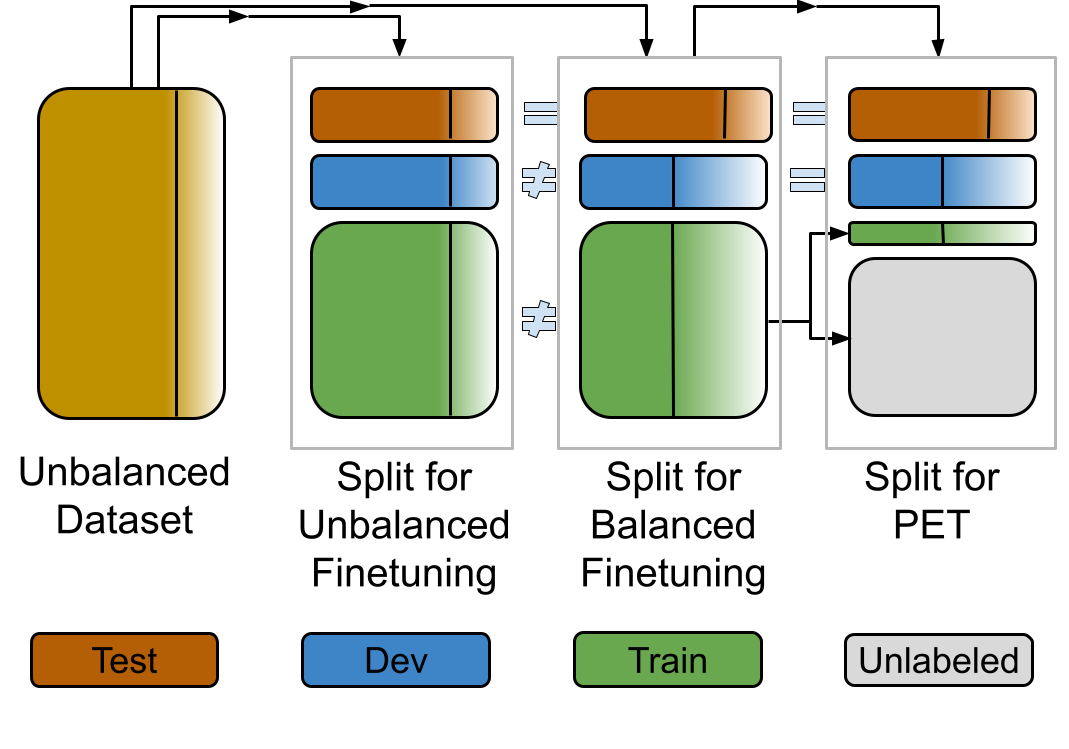
\includegraphics[width=0.5\textwidth]{Figures/06/06_dataset_splits.png}
    \caption{Strategies for Dataset Splitting}
    \label{fig:06_strategies_for_dataset_splitting}
\end{figure}